\documentclass[11pt,a4paper]{article}
\usepackage[margin=24mm]{geometry}
\usepackage{tikz}
\title{Canonical DE operator contracts and trace identity}
\date{Created 2026-09-29 20:59 CEST}
\begin{document}
\maketitle
\paragraph{Scope and ETA.} A compilable HyMeKo dependency description of the frozen
DE/rand/1/bin pilot, structural Query checks with negative cases, canonical
operator identity export, and identity binding to existing recorded events.
Estimate 40--60 minutes: source/validator, focused tests, recorded-trace binding,
documentation. No optimization campaign, simulation, external model call or Bat
reconstruction. Structural checks do not prove implementation equivalence.
\paragraph{Ownership.} Core's CompiledModel owns compilation, IR and semantic
identity; DerivedPathIndex owns canonical paths. Existing QueryEngine predicates,
effective fields, exact inheritance and match-count checks own structural query
semantics. A Formats research example owns DE-specific validation and JSON export.
The local pilot binds exported IDs without parsing HyMeKo. HySTL remains the only
temporal monitor and requires no semantic change.
\paragraph{Files.} New Formats example examples/metaheuristic\_contract.rs and
data/metaheuristics/de\_rand\_1\_bin.hymeko; focused tests embedded in that example.
The local docs/research/metaheuristics-pilot gains bind\_operator\_ids.py and
test\_operator\_ids.py; README, PROTOCOL and PROMPT receive precise integration notes.
The parent-approved optional prompt step adds build\_prompt\_inputs.py, extracting
an interface stub from the existing reference AST and assembling unsubmitted P/H
prompt bundles from the same frozen pseudocode and contract facts; its tests live
with the pilot identity checks. No provider is selected or invoked by this builder.
This four-file plan and reports/2026-09-29-metaheuristic-contract.md record provenance.
Generated contract JSON, DOT/SVG and a bound copy of an existing trace go under
the local pilot artifacts. No shared manifests, dependencies, Core, Tensor,
Kawamirai, adversarial-grid or existing overview/task files change.
\paragraph{Representation.} Explicit typed input/output dependency declarations
carry exact canonical state references. Source currently leaves PortDirection
unspecified; no direction is inferred from sign. Donor roles, old/new generation
state, boundary handling, equality replacement, budgets and random-decision
contract remain distinct. Export identity pairs the core semantic digest with the
core-derived canonical path; raw DeclIds are snapshot-local diagnostics only.
\paragraph{Validation.} Query checks assert vocabulary/profile uniqueness,
operator keys, input/output roles, state references and fixed DE profile values.
Negative fixtures cover missing/duplicate operator identity, omitted/wrong donor
dependency, reversed roles, foreign same-name types and semantic-profile drift.
Canonical emission/recompilation must preserve validated meaning and identity.
Python checks reject unknown event keys and registry/profile mismatch; they verify
recorded numeric data is unchanged. No graph interpreter is implemented.
\paragraph{Budget and risk.} One fixed small source, maximum 128 KiB, 4096
declarations and 128 operator roles for the input adapter. Query witnesses capped
at eight, no topology expansion or remote fetch by the fixture compiler. Work is
source-size bounded; tests target under 30 seconds after cached build. Existing
recorded trace binding is capped at 16 MiB input. No measured speedup or latency
claim is made. Canonical paths, not bare numeric IDs, avoid declaration-order
aliasing. The dirty Query owner is explicitly hashed; this is a local integration
until those changes are published. Duplicate framework revisions are checked with
cargo tree -d before edits.
\paragraph{State and rollback.} Reuse transformation feat/camera-perception,
HEAD 3421b4dabe4a173d52e64ed143db6544ab3e0165. Fetch all remotes succeeded;
HEAD equals fresh upstream and is seven commits ahead of origin/main. Preserve all
existing edits and both worktrees. CORE.YAML items touched: empty. No commit,
push, branch switch or new worktree. Rollback only this task's named new files
and its pilot documentation additions. Parent handles report archival.
\begin{center}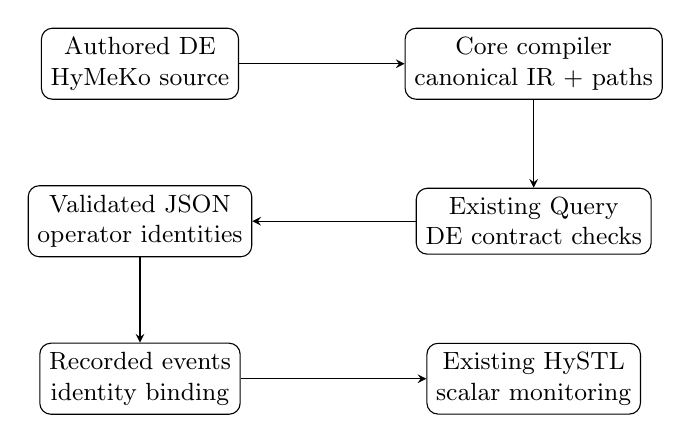
\begin{tikzpicture}[every node/.style={draw,rounded corners,align=center,font=\small},>=stealth]
\node (source) at (0,0) {Authored DE\\HyMeKo source};
\node (core) at (5,0) {Core compiler\\canonical IR + paths};
\node (query) at (5,-2) {Existing Query\\DE contract checks};
\node (ids) at (0,-2) {Validated JSON\\operator identities};
\node (events) at (0,-4) {Recorded events\\identity binding};
\node (stl) at (5,-4) {Existing HySTL\\scalar monitoring};
\draw[->] (source)--(core);
\draw[->] (core)--(query);
\draw[->] (query)--(ids);
\draw[->] (ids)--(events);
\draw[->] (events)--(stl);
\end{tikzpicture}
\end{center}
\end{document}
